\documentclass[a4paper,10pt]{article}
\usepackage[utf8]{inputenc}
\usepackage[colorlinks,plainpages=false]{hyperref}

\setlength\parindent{0pt}
\usepackage[english]{babel}
\usepackage[dvinames]{xcolor}
\usepackage[compact,small]{titlesec}
\usepackage{booktabs}
\usepackage{multirow}
\usepackage{amsfonts,amsmath,amssymb}
\usepackage{marginnote}
\usepackage[top=1.8cm, bottom=1.8cm, outer=1.8cm, inner=1.8cm, heightrounded, marginparwidth=2.5cm, marginparsep=0.5cm]{geometry}
\usepackage{enumitem}
\setlist{noitemsep,parsep=2pt}
\newcommand{\highlight}[1]{\textcolor{kuleuven}{#1}}
\usepackage{pythonhighlight}
\usepackage{cleveref}
\usepackage{graphicx}
\graphicspath{{Pictures/}}
\usepackage{algorithmic}
\usepackage{tabularx}
\usepackage{bm}
\usepackage{subcaption}
\usepackage{array}


\newcommand{\nextyear}{\advance\year by 1 \the\year\advance\year by -1}
\newcommand{\thisyear}{\the\year}
\newcommand{\deadlineGroup}{November 27, \thisyear{} at 16:00 CET}
\newcommand{\deadlineCode}{December 18, \thisyear{} at 16:00 CET}
\newcommand{\deadlineReport}{January 4, \nextyear{} at 16:00 CET}

\newcommand{\ReplaceMe}[1]{{\color{blue}#1}}
\newcommand{\RemoveMe}[1]{{\color{purple}#1}}

\setlength{\parskip}{5pt}

%opening
\title{Artificial Neural Networks: Exercise session 4}
\author{Stijn Staring (r0620003)}

\begin{document}
\fontfamily{ppl}
\selectfont{}

\maketitle


\section{Restricted Boltzmann Machines}
The Boltzmann machine is a parametrized generative model representing a probability distribution. It is a neural network that belong to energy based models. A Boltzmann Machine consist out of a layer of visible units $ \bm{v} $ and hidden units $ \bm{h} $. The energy function used by the model is shown in Eq. \ref{eq:1a} and is part of the joint probability distribution. The standard type of Boltzmann Machines, uses binary-valued hidden and visible units and is therefore convenient to be used for black white images. The difference between a Restricted Boltzmann Machine and a conventional  Boltzmann Machine, is that the units of one layer are not connected with each other. Because of this restriction, the partition function in the joint probability distribution seen in Eq. \ref{eq:1b} becomes tractable. A RBM trains in an unsupervised manner using only the observations and calculating the gradient of the log-likelihood of the observations with respect to the weight matrix $ \bm{W} $, and bias terms $ \bm{a} $ and $ \bm{b} $. Training a RBM means adjusting the RBM weight values and  biases such that the probability distribution $ P(\bm{v}) $ fits the training data as well as possible. The gradient of the log-likelihood is calculated by the difference between the data expectation and model expectation and is used together with a learning rate and a gradient decent update strategy. However, because the calculation of the model expectation is intractable, the Contrastive Divergence algorithm is used. Gibbs sampling is applied to generate an observation from the model distribution and is used in the Contrastive Divergence algorithm. Gibbs sampling is initialized by a known observation

\begin{subequations}
	\begin{equation}\label{eq:1a}
		E(\bm{v},\bm{h}) = -\bm{v}^T\bm{W}\bm{h} - \bm{b}^T\bm{v}-\bm{a}^T\bm{h},
	\end{equation}
	\begin{equation}\label{eq:1b}
		P(\bm{v},\bm{h}) = \frac{1}{Z}e^{-E(\bm{v},\bm{h})}    .
	\end{equation}
	\label{eq:1}
\end{subequations}

\subsection{Hyperparameter tuning}
A small hyperparameter tuning is displayed in Table \ref{tab:pseudo-likelihood}. It is seen that more iterations give better results. When looking at the column with 20 iterations, an U-shape is noticed in the pseudo-likelihood. For a small learning rate of $ 0.005 $ a larger error is found due to the slow convergence and a larger learning rate of $ 0.1 $ performs worse due to oscillations during the application of gradient descent. The use of more hidden units gives an higher likelihood of the observations. Using more iterations and hidden units increases the calculation load of the model. The final chosen values for the parameters are $ 20 $ iterations, $ 20 $ hidden units and a learning rate of $ 0.01 $. In Figure \ref{fig:hyperpara} the comparison on the reconstruction of the number 4 is given with the tuned parameters and the default ones. It shows that the tuned RBM is able to better reconstruct an image with deleted row than when using the default parameter values that uses $ 10 $ iterations, $ 10 $ hidden units and a learning rate of $ 0.01 $ during training. 

\begin{table}[h]
	\begin{minipage}[t]{.55\linewidth}
		\centering
			\begin{tabular}[t]{@{}l|ccc}
				\firsthline
				\textbf{Learning rate}/\textbf{Iterations}	&  5 & 10 & 20 \\ \midrule
				0,005&	-141	&-134&	-127,41	\\ \hline
				0,01&	-166&	-147,66&	-125,55\\ \hline
				0,05 &	-141,15&	-134,35&	-127,41\\ \hline
				0,1 &	-134,46&	-130,24&	-130,81\\\bottomrule
			\end{tabular}		
	\end{minipage}
	\begin{minipage}[t]{.45\linewidth}
		\centering
		\begin{tabular}[t]{@{}l|ccc}
			\firsthline
			\textbf{Iterations}/\textbf{Hidden units}	&  5 & 10 & 20 \\ \midrule
			5 &-185	&-155,08&	-134,46	\\ \hline
			10&	-186	&-154&	-130\\\bottomrule
		\end{tabular}
	\end{minipage} 
	\caption{Pseudo-likelihood on the training data when training with different parameter values.}
	\label{tab:pseudo-likelihood}
\end{table}

\subsection{Gibbs sampling}
In Gibbs sampling it is started from an initial known observation $ \bm{v}^{(1)} $ and by the sequential use of $ P(\bm{h}|\bm{v}^{(1)}) $ and $ P(\bm{v}|\bm{h}^{(1)}) $, one iteration of the Gibbs sampling is completed and a new observation is obtained. A property of Gibbs sampling is that only after a infinite amount of iterations it can be guaranteed that the generated sample originates from the model probability distribution that is tried to be sampled from. As can be seen in Figure \ref{fig:gibbssampeling} after one iteration the original number 2 is still visible but after 100 iterations it is not recognizable anymore. The influence of the initial observation is reduced after 100 iterations and the obtained observation will correspond better to one that  originates from the model probability distribution. 

\begin{figure}[ht]
	\begin{subfigure}{0.32\textwidth}
		\centering
		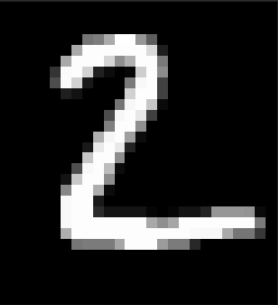
\includegraphics[width=0.5\linewidth]{0iter_gibbs.png}
		\caption{Original}
		\label{fig:0iter}
	\end{subfigure}	 	
	\begin{subfigure}{0.32\textwidth}
		\centering
		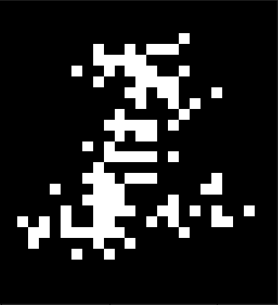
\includegraphics[width=0.5\linewidth]{1iter_gibbs.png}
		\caption{1 iteration}
		\label{fig:1iter}
	\end{subfigure}	
	\begin{subfigure}{0.32\textwidth}
		\centering
		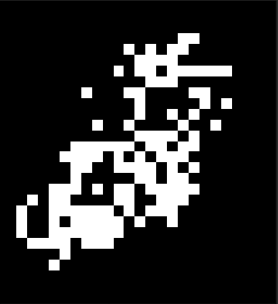
\includegraphics[width=0.5\linewidth]{100iter_gibbs.png}
		\caption{100 iterations}
		\label{fig:100iter}
	\end{subfigure}
	\caption{The effect of iterations of Gibbs sampling.}
	\label{fig:gibbssampeling}
\end{figure}


\subsection{Reconstructing images}
The general rule in reconstructing images is that when more information is missing from the original image, it is harder to reconstruct. Deleting more information can be done by deleting more rows or deleting crucial places that play a key role in distinguishing the number. Figure \ref{fig:hyperpara} shows the reconstruction of the number 4 using the default RBM and tuned RBM when rows 10 till 15 are removed. The tuned model shows better results. In order to reconstruct the image, the image with deleted rows is feeded as observed example to the trained RBM and Gibbs sampling is applied. An observation is retrieved from the model probability distribution and the corresponding rows are used to fill the gap of the original image. For both images 10 Gibbs sampling steps are used.

\begin{figure}[h]
	\begin{subfigure}{0.49\textwidth}
		\centering
		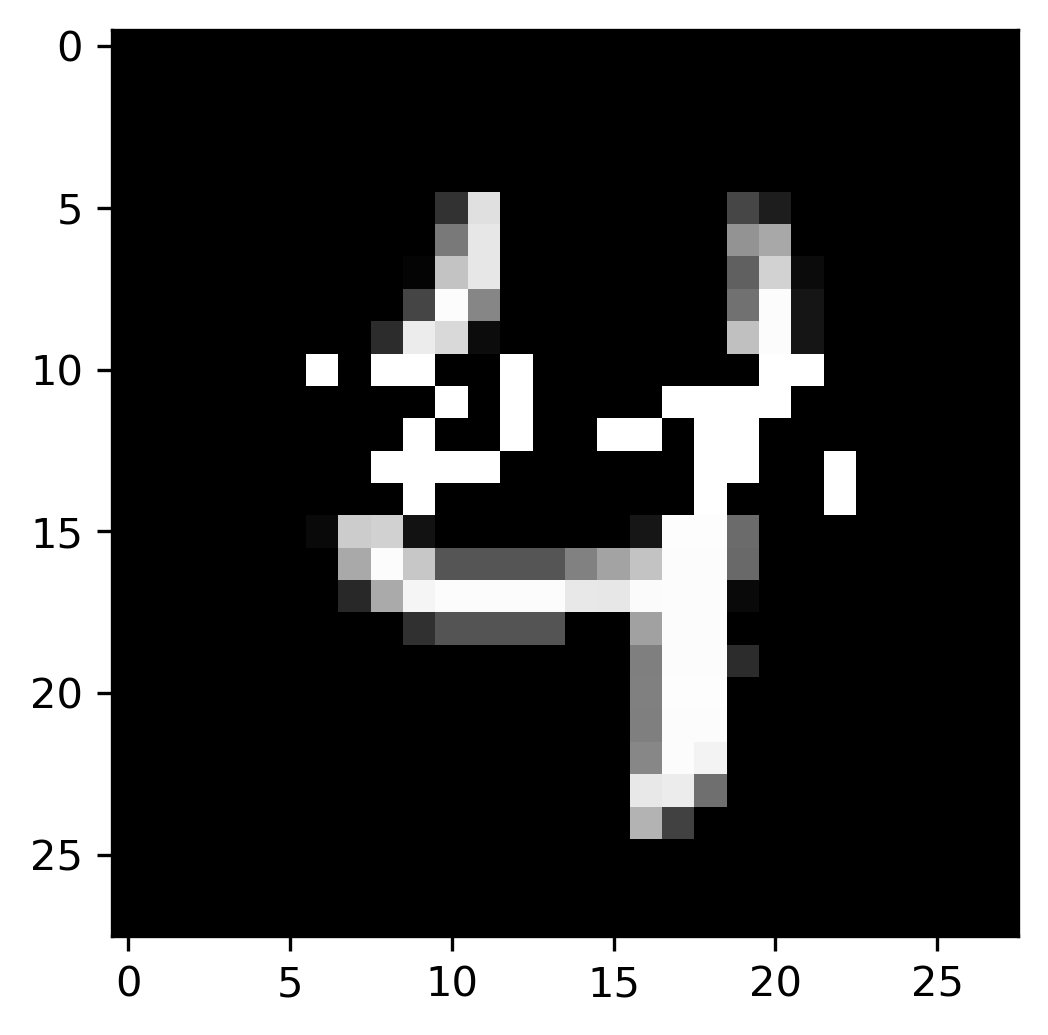
\includegraphics[width=0.4\linewidth]{default.png}
		\caption{Default}
		\label{fig:default}
	\end{subfigure}	 	
	\begin{subfigure}{0.49\textwidth}
		\centering
		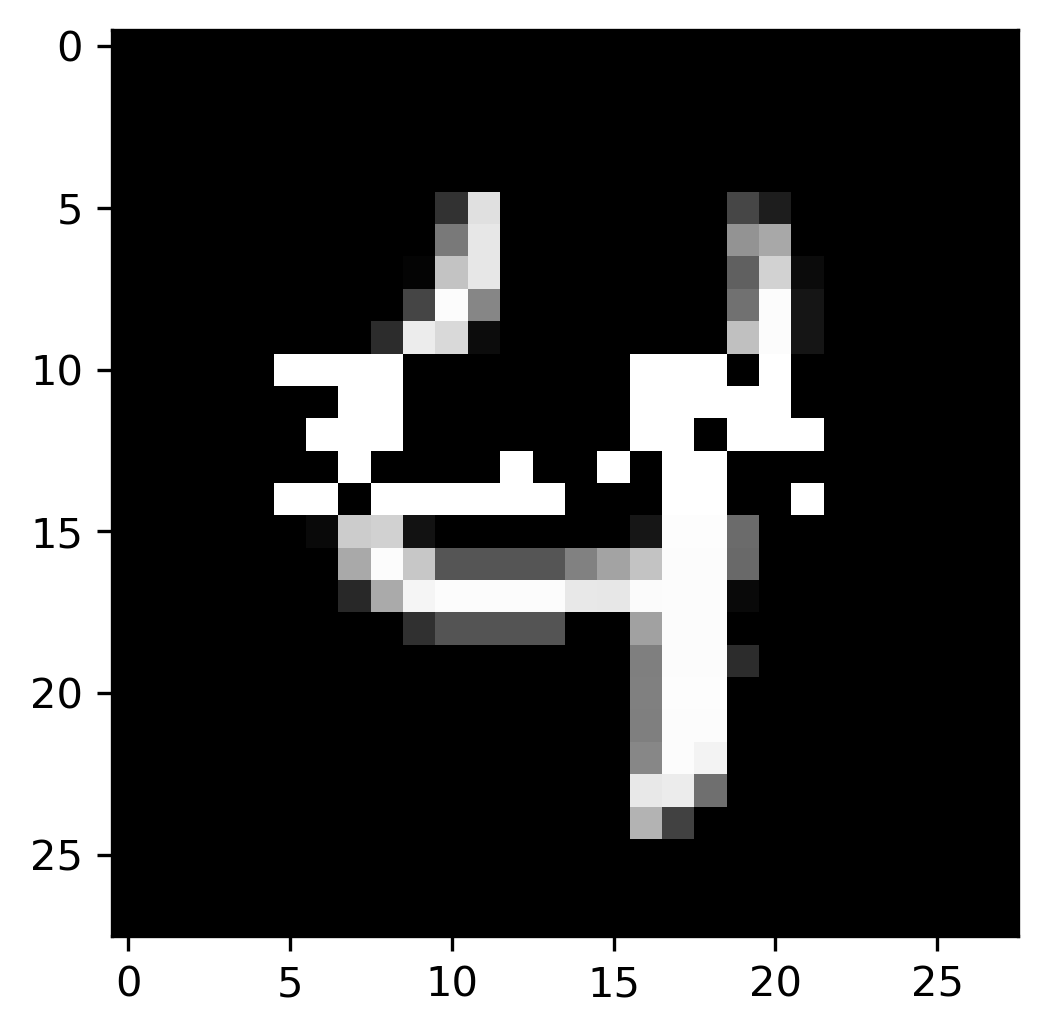
\includegraphics[width=0.4\linewidth]{tuned.png}
		\caption{Tuned}
		\label{fig:tuned}
	\end{subfigure}	
	\caption{The effect of hyper parameter tuning.}
	\label{fig:hyperpara}
\end{figure}

\section{Deep Boltzmann Machines}




%\begin{table}
%	\centering
%	\begin{tabular}{@{}clr@{}} \toprule
%		\textbf{Attractor} & \textbf{Point} & \textbf{Stability}\\\midrule
%		Attractor $ 1 $ & $ [1;1] $ & Stable\\
%		Attractor $ 2 $ & $ [-1;-1] $ & Stable\\
%		Attractor $ 3 $ & $ [1;-1] $ & Stable\\
%		Attractor $ 4 $ & $ [-1;1] $ & Stable\\
%		Attractor $ 5 $ & $ [0;0] $ & Unstable\\
%		Attractor $ 6 $ & $ [0;1] $ & Unstable\\
%		Attractor $ 7 $ & $ [0;-1] $ & Unstable\\
%		Attractor $ 8 $ & $ [1;0] $ & Unstable\\
%		Attractor $ 9 $ & $ [-1;0] $ & Unstable\\\bottomrule
%	\end{tabular}
%	\caption{Overview of the different attractor points found in a 2D plane.}
%	\label{tab:att}
%\end{table}

\bibliographystyle{abbrv}
%\bibliography{ANN1}

\end{document}
